\chapter{Main controller}
\section{Inleiding}
De main controller bevat de interface van de wekker. Deze zorgt er voor dat een wekker ingesteld kan worden, aangepast kan worden en uitgezet kan worden. 
Belangrijk aan elke interface is dat deze gebruiksvriendelijk is. 
Dit kan onder andere bereikt worden door een optimum voor het aantal knoppen te bepalen. 
Te veel knoppen, en de gebruiker weet niet welke knop wat doet, te weinig knoppen, en de gebruiker moet navigeren door een nodeloos ingewikkeld menu. \\
Daarnaast is er nog een beperkende factor: het aantal pinnen op de chip. \\
Al deze informatie samengenomen is besloten dat 4 knoppen voor de interface het meest gebruiksvriendelijke resultaat oplevert. Daarnaast is er nog een knop die slechts gebruikt wordt om een afgaand alarm uit te zetten. \\
De controller stuurt een hoop dingen aan, en van te voren was al geanticipeerd dat dit hierdoor een van de grootste onderdelen op de chip zou kunnen worden.

\section{Specificaties}
\subsection{Ingangen}
\begin{itemize}[nolistsep]
\item Klok, dit is een standaard input;
\item Reset, ook dit is een standaard input;
\item Knoppen, dit zijn de 4 knoppen die (nadat ze gebufferd zijn) onderdeel zijn van de interface.
\begin{itemize}[nolistsep]
\item knoppen[0] = menu
\item knoppen[1] = set 
\item knoppen[2] = up
\item knoppen[3] = down\\
\end{itemize}
\end{itemize}



\subsection{Uitgangen}
\begin{itemize}[nolistsep]
\item Wekker, dit is de tijd dat de wekker af moet gaan en de wekkerdata, dus of het licht en geluid aan staan, en of de wekker uberhaupt aanstaat;
\item Menu-state, dit is de staat in welke de FSM zich op het moment bevindt. Deze informatie wordt doorgevoerd naar het LCD-scherm om zo te kunnen zien waar in het menu men zit.\\
\end{itemize}
In \cref{tab:uitgangen_controller} staat wat voor informatie te vinden is in de uitgangen van de controller.
\begin{table}[ht!]
\caption{Uitgangen van de controller}
\label{tab:uitgangen_controller}
\begin{tabular*}{\textwidth}{@{\extracolsep{\fill} }|l| p{.75\textwidth}|}
\hline
Uitgang & Informatie over wat in de uitgang te vinden is \\ \hline
wekker & De huidige info over de wekker instellingen uit geheugen \newline
wekker[5 down to 0] daarin staan de minuten \newline
wekker[10 down to 6] daarin staan de uren \newline
wekker[11] geluid bit \newline
wekker[12] led bit \newline
wekker[13] wekker bit (Of de wekker uberhaupt aan is of niet) \\ \hline
menu & Deze geeft door aan de in welke state we zitten aan de lcd module \newline
000 : Het normale scherm weergeven met alarm en wekkertijd weergave state: Rust,Wekkertijd \newline
001 : Uren aanpassen \newline
010 : Minuten aanpassen \newline
011 : Led aanpassen \newline
100 : Geluid aanpassen \\ \hline
\end{tabular*}
\end{table}
\newpage
\subsection{Gedrag}
Om te beginnen moet de tijd waarop de wekker af moet gaan ingesteld kunnen worden. Dit wordt gedaan door eerst de huidige wekkertijd weer te geven, vervolgens het uur waarop gewekt moet worden te wijzigen en daarna de minuut. Hierna wordt de huidige tijd weer weergegeven. \\
Daarnaast is een vereiste dat de led uitgezet moet kunnen worden. Afhankelijk van een instelling moet het wake-up-light gedeelte wel of niet aangaan. Hetzelfde geld voor het geluid. \\
Dit alles moet zo gebruiksvriendelijk mogelijk gebeuren.

\section{Functionaliteit}

\subsection{FSM}
In \cref{fig:FSM_controller} staat de gemaakte fsm en in \cref{tab:states_controller} staan de uitgangen per state gespecificeerd.

\begin{figure}[ht!]
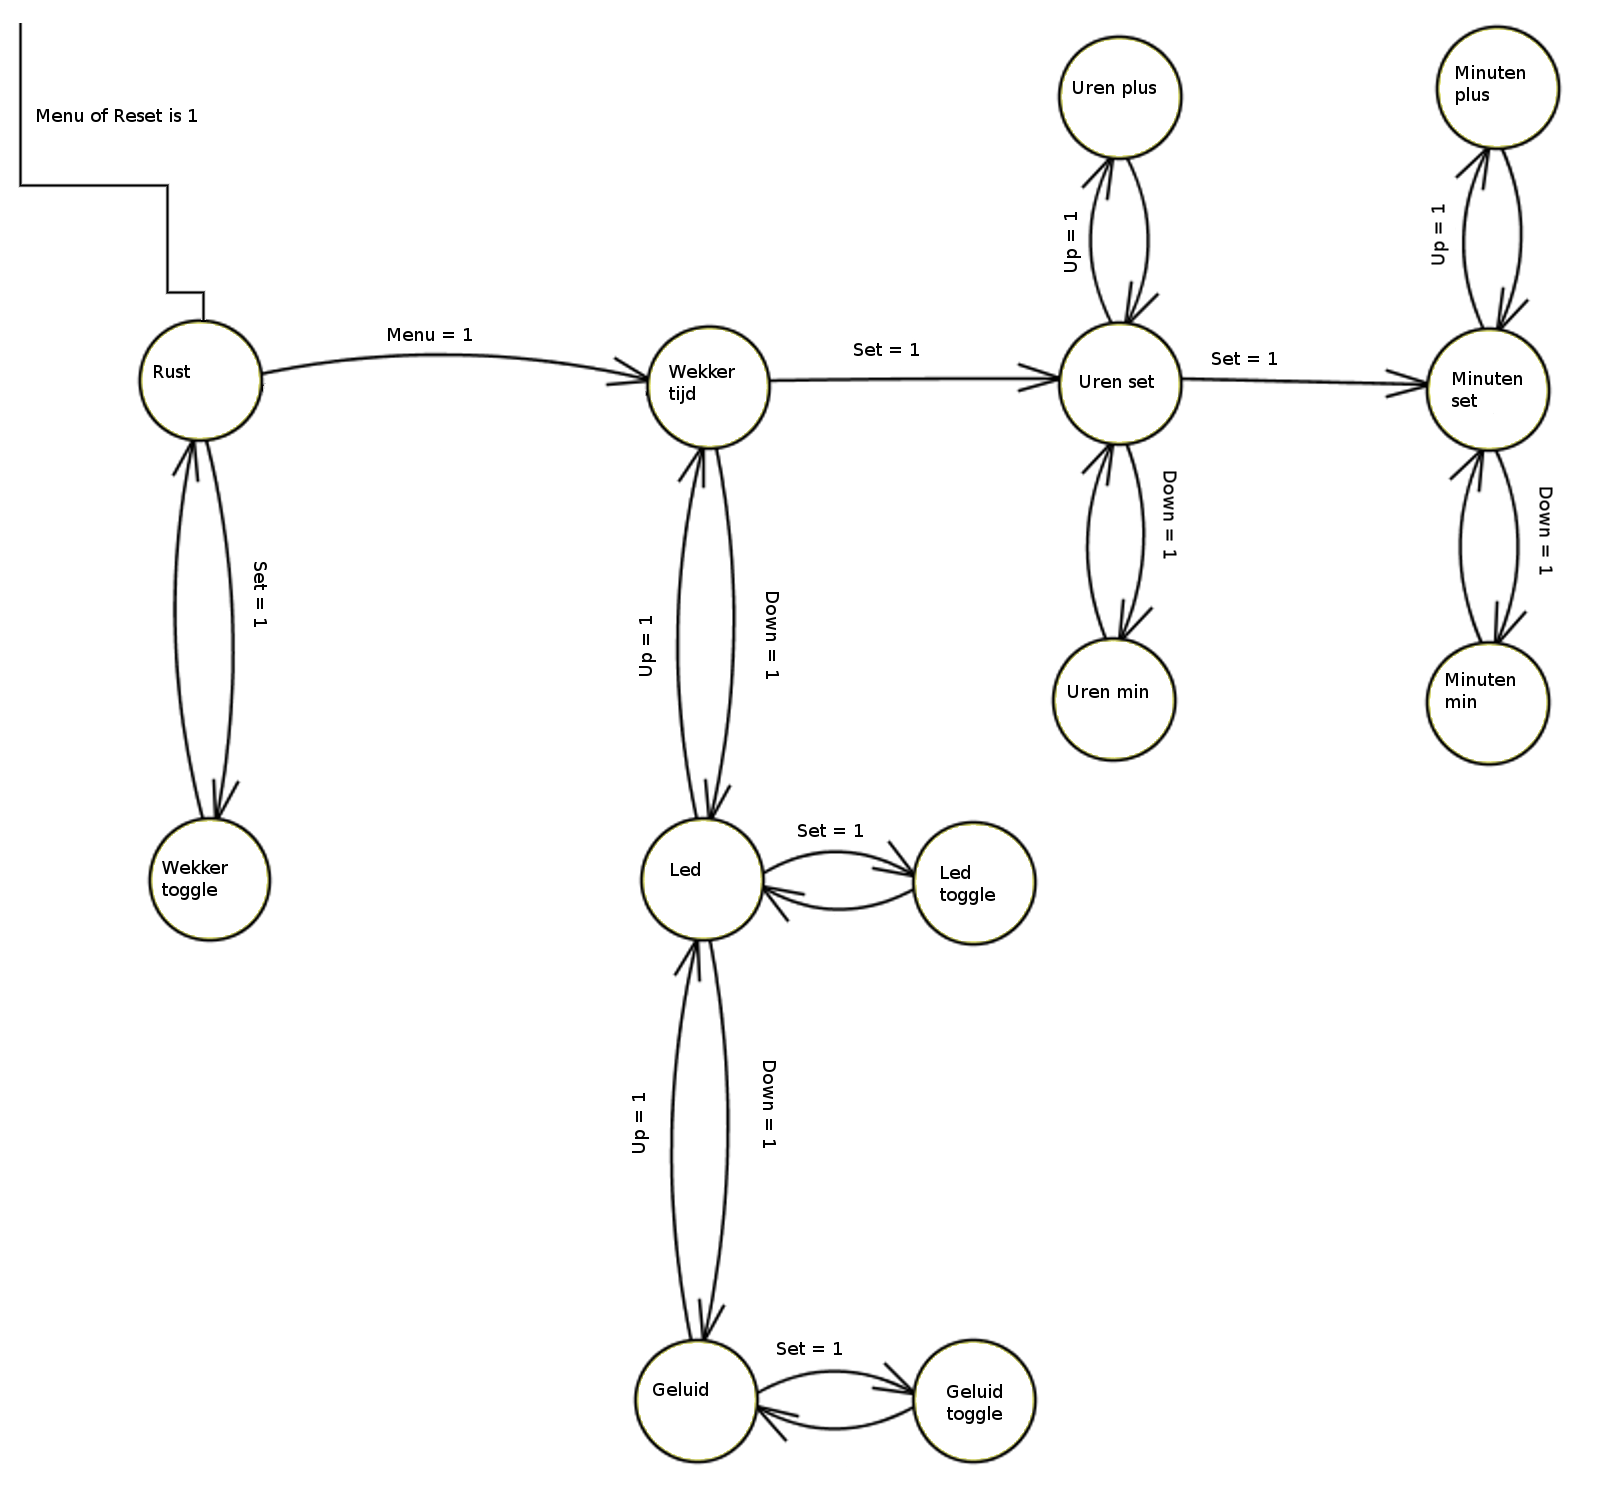
\includegraphics[width=\textwidth,height=\textheight,keepaspectratio]{Figuren/Controller/FSM_controller.png}
\caption{FSM diagramma van de menu}
\label{fig:FSM_controller}
\end{figure}

\begin{longtable}{|l| p{10cm} |}
\hline
Rust &
enable = '0' \newline
wekker=wekdata \newline
menu= "000" \\ \hline
Wekker toggle &
enable = '1' \newline
wekker[12 down to 0]=wekdata[12 down to 0] \newline
wekker[13]= niet wekdata[13] \newline
menu = "000" \\ \hline
Wekkertijd &
enable ='0' \newline
wekker=wekdata \newline
menu = "000" \\ \hline
Led &
enable ='0' \newline
wekker=wekdata \newline
menu = "011" \\ \hline
Led toggle &
enable ='1' \newline
wekker[11 down to 0]=wekdata[11 down to 0]\newline
wekker[12] = niet wekdata[12] \newline
wekker[13] = wekdata[13] \newline
menu = "011" \\ \hline
Geluid & 
enable ='0' \newline
wekker=wekdata \newline
menu = "100" \\ \hline
Geluid toggle &
enable ='1' \newline
wekker[10 down to 0]=wekdata[10 down to 0] \newline
wekker[11] = niet wekdata[11] \newline
wekker[13 downto 12] = wekdata[13 downto 12] \newline
menu = "100" \\ \hline
Uren set &
enable ='0' \newline
wekker=wekdata \newline
menu = "001" \\ \hline
Uren plus &
enable ='1' \newline
wekker=wekdata+1 \newline
menu = "001" \\ \hline
Uren min &
enable ='1' \newline
wekker=wekdata-1 \newline
menu = "001" \\ \hline
Minuten set&
enable ='0' \newline
wekker=wekdata \newline
menu = "010" \\ \hline
Minuten plus &
enable ='1' \newline
wekker=wekdata+1 \newline
menu = "010" \\ \hline
Minuten min &
enable ='1' \newline
wekker=wekdata-1 \newline
menu = "010" \\ \hline
\caption{Uitgangen binnen de state van de controller} 
\label{tab:states_controller}
\end{longtable}

\subsection{VHDL code}
De code voor de controller van de wekker is te vinden in \cref{Ap:code_controller}. Voor de overzicht en het modular opbouwen is de code in vier blokken geschreven.
\begin{itemize}[nolistsep]
\item De top entity met de port map. Deze is te vinden in \cref{code:controller_ent,code:controller_beh}.
\item Het menu, hierin zit de echte logica verwerkt. Deze is te vinden in \cref{code:menu_ent,code:menu_beh}.
\item Het gebruikte geheugen element voor de opslag van 14 bits, te vinden in \cref{code:geheugen_ent,code:geheugen_beh}.
\item De gebruikte buffer is te vinden in \cref{code:buffer_ent,code:buffer_beh}. De buffer regelt het ingangssignaal, en zorgt ervoor dat er maar 1 klokperiode lang een hoog signaal gelezen word.
\end{itemize}
Voor het testen van de code zijn er testbenches gemaakt welke te vind zijn in \cref{code:tb_controller,code:tb_menu,code:tb_geheugen,code:tb_buffer}.

\section{Testen}
Om zeker te zijn dat alles goed werkt worden er drie verschillende testen uitgevoerd. De eerste is op behavioural niveau. Hier wordt getest of de basis van de code werkt zoals verwacht. Na een goed geslaagd resultaat kan de code worden gesynthetiseerd, en deze gesynthetiseerde code worden gesimuleerd. Als er geen fouten optreden kan het ontwerp gemaakt worden, daarna geextraheerd en nogmaals getest worden. De testen worden uitgevoerd met behulp van \emph{Modelsim}.


\section{Simulatie}
De resultaten van de simulatie staan in \cref{Ap:sim_controller}. De testbench is te lang om in een keer weer te geven daarom is deze op geknipt in vier stukken. De testbench die gemaakt is voor de simulatie staat in \cref{code:tb_controller}
\section{Resultaten}
Van \cref{fig:sim_beh_0-2_5} tot en met \cref{fig:sim_ext_7_5-} is te zien dat iedere simulatie tot hetzelde resultaat leid en daarmee succesvol is.
De minimale klokperiode kan afgelezen worden aan de hand van \cref{fig:timing_controller}. Hieruit is op te makken dat deze 60ns is.
\subsection{Conclusie en discussie}
De controller werkt op alle gesimuleerde niveau's naar verwachting. 
De minimale klok periode bedraagt 60ns om gliches te voorkomen bij het optellen en aftrekken van uren en minuten. 
De controller maakt op dit moment gebruik van 9088 transitoren waarvan er voor de daadwerkelijke schakelingen slechts 2914 worden gebruikt. 
De controller maakt op dit moment nog gebruik van het binaire telsysteem (dat gebruik maakt van machten van 2), er bleek echter dat voor de lcd scherm BCD veel beter werkt. Dit moet nog worden geimplementeerd. Vlak nadat het inputbuffer gemaakt was kwam men er achter dat in plaats van een buffer ook de rising\textunderscore edge functie gebruikt had kunnen worden. 

